\documentclass[11pt]{article}
\usepackage[margin=1in]{geometry}
\usepackage{booktabs,graphicx,microtype,amsmath}
\usepackage[numbers,sort&compress]{natbib}
\usepackage[hidelinks]{hyperref}
\setlength{\parskip}{0.35em}
\renewcommand{\arraystretch}{1.12}

\title{Repairing Multi-Key Recall in Converted Hybrid Language Models}
\author{Musaab Mahjoub\\ Aalborg University, Denmark\\ \texttt{musab.ahmed1996@gmail.com}}
\date{October 2026}

\begin{document}
\maketitle

\begin{abstract}
A hybrid language model replaces most attention layers with linear layers that keep a fixed-size state. Converting a trained transformer into a hybrid is cheap. We ask what the conversion loses and whether it can be put back.
We plant 16 facts in documents of 1K to 32K tokens and ask for one. Two converted hybrids, Jet-Nemotron-2B and an 8B Mamba-in-the-Llama, answer a single-needle test perfectly at every length and recall one of 16 facts at 32K with rates of 0.31 and 0.25. The models they were converted from recall at 0.90 and 0.99. RULER's multi-key tasks show the same gap.
A low-rank adapter on under 1\% of the weights, trained for 40 minutes on one GPU with synthetic many-fact documents, restores recall to the source model's level: 1.00 at 2B and 0.99 at 8B, replicated over three seeds each. The 8B repair is trained at 16K and holds at 32K. It transfers to RULER's numeric multi-key tasks and to a template never trained on. It does not transfer to UUID values, and it loses two-hop questions unless the training data contains them. The repair learns exactly the retrieval it is shown.
The cost is measurable. At 2B, long-text bits per byte rise 0.4\%. At 8B the 2B dose over-fits (+15\%); a quarter dose gives full recall at +6\%, and natural-text replay removes the cost but also removes two-hop recall. We give the recipe, its boundaries, and the harness.
\end{abstract}

\section{The question}
A transformer stores every token it reads. A linear-attention layer folds what it reads into a matrix of fixed size. Hybrids keep a few attention layers and make the rest linear, and so cost far less memory per long request. Several recipes convert an existing transformer into a hybrid by distillation \citep{mambainllama2024,lolcats2024,radlads2025,jetnemotron2025}. Their papers report language-modelling benchmarks and, when they report long context, a single-needle test or an aggregate score.

Two things are already known. Linear states lose associative recall as the number of facts and the distance grow \citep{zoology2023,based2024,waleffe2024,stuffedmamba2024}. And a single needle is the easiest case for a fixed state, which is why RULER \citep{ruler2024} tests several needles at once.

We ask three narrower questions about converted models.
\begin{enumerate}
\item Does a converted hybrid lose multi-key recall relative to the exact model it was converted from, while passing the single-needle test?
\item If it does, is the state too small, or merely untrained? A small post-hoc adapter answers this: if training restores recall, the capacity was there.
\item What does the repair cost, and what does it not fix?
\end{enumerate}

\section{The test}
\paragraph{Documents.} A document is filler text with planted sentences. Filler is drawn from a bank of $32^3$ combinatorial sentences about office logistics and contains no digits. A planted sentence reads \emph{The access code for locker KX-402 is 481930.} Values are six-digit codes, so a code in the answer can only come from a planted sentence or be invented. Documents are sized under one reference tokenizer (Qwen2.5) to 1K, 2K, 4K, 8K, 16K and 32K tokens, within 1.3\% of target. Every model sees byte-identical prompts.

\paragraph{Tasks.} Five tasks, 25 cases per task and length:
\begin{itemize}
\item \textbf{needle}: one key, one fact. The control.
\item \textbf{16 random keys}: sixteen facts with unrelated keys; ask for one.
\item \textbf{16 similar keys}: sixteen facts whose keys differ in one digit (KX-401 to KX-416); ask for one.
\item \textbf{updated}: eight keys, each assigned a code and later changed; ask for the current code.
\item \textbf{multi-hop}: eight chains, locker $\to$ person $\to$ code; ask for the code of the person assigned to a locker.
\end{itemize}
A held-out task, \textbf{parcels}, plants sixteen facts with a different template (\emph{Parcel 48213-K has the pickup code 731902.}). It is never used for training.

\paragraph{Prompting and scoring.} Completion style, no chat template: an instruction, the document, the question, and \emph{Answer:}. Greedy decoding, 32 new tokens. Models with a \texttt{<think>} token get the empty reasoning block prefilled. A case counts as recalled if the planted code appears among the six-digit numbers on the first visible line of the completion. Generation is deterministic: 150 of 150 completions were byte-identical across two runs on the same GPU type.

\paragraph{RULER.} We also run NVIDIA's RULER needle variants, generated with their own code and the same tokenizer: single needle, three multi-key variants, multi-value and multi-query, 50 cases each at 16K and 32K, scored by their rule (every expected string anywhere in the output).

\section{What converted models do}
\paragraph{Models.} Two matched pairs.
Jet-Nemotron-2B \citep{jetnemotron2025} keeps 2 full-attention and 2 sliding-window layers of 28 and replaces the rest. It was initialised from Qwen2.5-1.5B; its conversion then trained the whole model for 350B tokens, so Qwen2.5-1.5B is the initialisation checkpoint, not a weight-identical base.
Mamba-in-the-Llama 8B \citep{mambainllama2024} replaces half the layers of Llama-3.1-8B-Instruct \citep{llama3_2024} with Mamba-2 layers \citep{mamba2_2024}.

\paragraph{Result.} Figure~\ref{fig:signature} and Table~\ref{tab:signature}. Both hybrids answer the needle at 1.00 at every length, as do their sources. On 16 keys the hybrids fall with length and the sources do not. At 2B the gap opens at 16K. At 8B it opens at 4K and is near total at 32K.

\begin{figure}[t]
\centering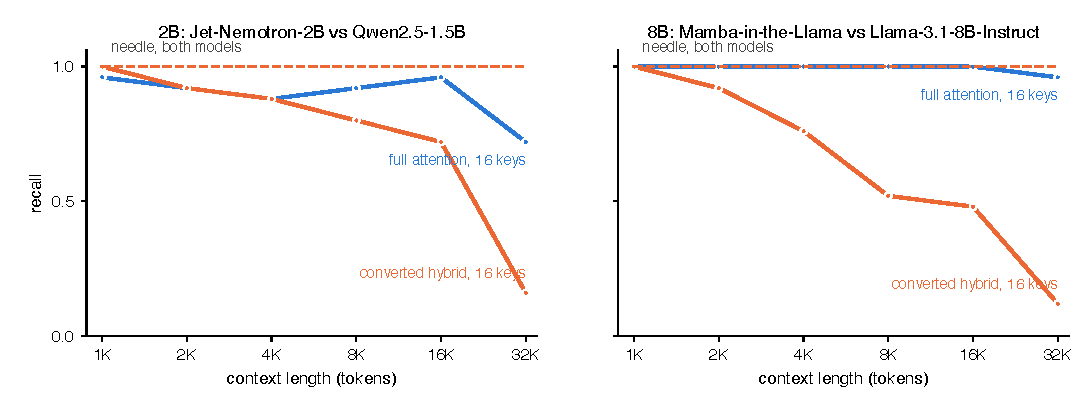
\includegraphics[width=\linewidth]{fig/fig1_signature.pdf}
\caption{Recall against context length, 25 cases per point. Dashed: a single needle. Solid: one of 16 random keys. Each converted hybrid is paired with the model it was converted from.}
\label{fig:signature}
\end{figure}

\begin{table}[t]
\centering\footnotesize\setlength{\tabcolsep}{3.5pt}
\caption{Recall at 32K with 100 fresh cases per cell (two suites of 50), and RULER multi-key at 32K with 50 cases. MK1--3: RULER multikey 1--3; MV, MQ: multi-value, multi-query.}
\label{tab:signature}
\begin{tabular}{lccccccccc}
\toprule
 & needle & 16 random & 16 similar & multi-hop & parcels & MK1 & MK2 & MK3 & MV \\
\midrule
Qwen2.5-1.5B, source & 1.00 & 0.90 & 0.75 & 0.14 & 0.94 & 0.94 & 0.72 & 0.40 & 0.46 \\
Jet-Nemotron-2B, hybrid & 0.86 & 0.31 & 0.22 & 0.11 & 0.45 & 0.56 & 0.26 & 0.16 & 0.02 \\
\addlinespace
Llama-3.1-8B-Instruct, source & 1.00 & 0.99 & 1.00 & 0.49 & 1.00 & 1.00 & 1.00 & 0.96 & 0.98 \\
Mamba-in-the-Llama 8B, hybrid & 1.00 & 0.25 & 0.09 & 0.06 & 0.17 & 0.40 & 0.10 & 0.00 & 0.00 \\
\bottomrule
\end{tabular}
\end{table}

Three details matter. The misses are well formed: the model returns another planted code in a correct sentence. RULER's multi-key tasks detect the same failure, so our harness adds no detection power over RULER; its contribution is the paired measurement and what follows. And near-duplicate keys were no harder than random keys below 32K, against our expectation that key geometry would be the main stressor.

\section{The repair}
\paragraph{Training data.} Synthetic documents in the locker template only, 16 to 48 planted keys, in four kinds cycled evenly: random keys, near-duplicate keys, keys overwritten once, and two-hop chains. Each document ends with eight questions. Loss is taken on the answer tokens only. The output head is applied only at those positions, which keeps 16K-token documents within one GPU's memory.

\paragraph{Adapter.} LoRA \citep{lora2021}, rank 16, on every linear projection outside the MLPs: the attention projections and the linear-attention projections. At 2B this is 232 layers and 0.75\% of the weights; at 8B, 96 layers and 0.15\%. AdamW, four documents per step. Two doses: \emph{heavy}, 600 documents at learning rate $2\times10^{-4}$; \emph{gentle}, 300 documents at $5\times10^{-5}$. The 2B model trains on 8K, 16K and 32K documents; the 8B model on 8K and 16K only, so its 32K numbers test generalisation past the trained length. The heavy 2B run takes 42 minutes on one A100-40GB. The adapter is merged into the weights, so inference cost is unchanged; merged and unmerged give identical scores.

\paragraph{Control.} The same recipe is applied to the full-attention source model. A gain that appears in both is familiarity with the format. A gain only in the hybrid is repair.

\paragraph{Result.} Figure~\ref{fig:repair} and Table~\ref{tab:repair}. At 2B, three seeds of the heavy recipe take 16-key recall at 32K from 0.31 to 1.00, 0.98 and 1.00, the level of the trained control. At 8B, three seeds of the gentle recipe, trained at 16K and below, give 1.00, 1.00 and 0.99 at 32K, the level of Llama-3.1-8B-Instruct. The held-out parcel template, never trained on, reaches 0.93 to 0.98 at 2B and 0.98 to 1.00 at 8B.

\begin{figure}[t]
\centering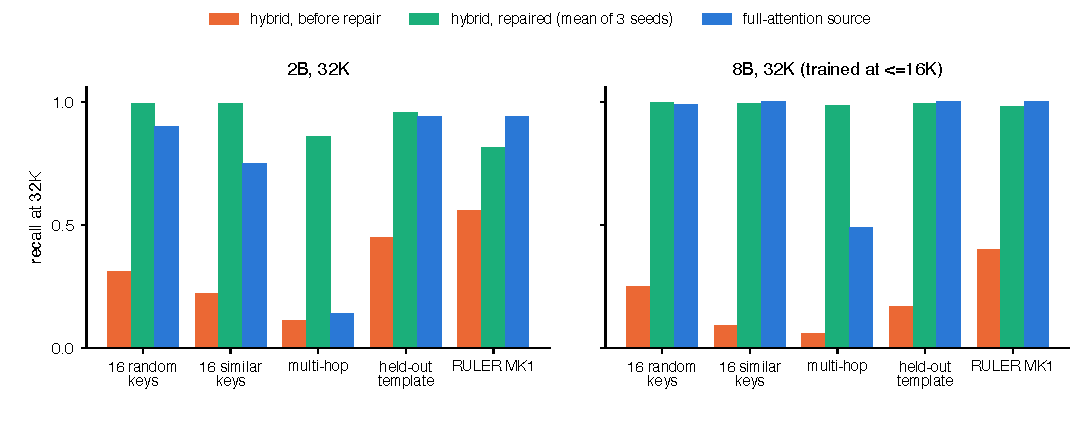
\includegraphics[width=\linewidth]{fig/fig2_repair.pdf}
\caption{Recall at 32K before and after repair, next to the full-attention source. Repaired bars are the mean of three training seeds. The 8B adapter never saw a 32K document.}
\label{fig:repair}
\end{figure}

\begin{table}[t]
\centering\small
\caption{Repair, 32K, 100 cases per cell; RULER 50 cases. Hybrid values are means over three seeds. The control is the source model trained with the same recipe (2B only; at 8B the source was not retrained).}
\label{tab:repair}
\begin{tabular}{llccccccc}
\toprule
 & & 16 random & 16 similar & multi-hop & parcels & MK1 & MK2 & MV \\
\midrule
2B & hybrid before & 0.31 & 0.22 & 0.11 & 0.45 & 0.56 & 0.26 & 0.02 \\
   & hybrid repaired & 0.99 & 0.99 & 0.86 & 0.96 & 0.81 & 0.49 & 0.12 \\
   & source trained (control) & 1.00 & 0.96 & 0.99 & 0.99 & 0.96 & 0.97 & 0.37 \\
\addlinespace
8B & hybrid before & 0.25 & 0.09 & 0.06 & 0.17 & 0.40 & 0.10 & 0.00 \\
   & hybrid repaired (gentle) & 1.00 & 0.99 & 0.99 & 0.99 & 0.98 & 0.89 & 0.73 \\
   & source, untrained & 0.99 & 1.00 & 0.49 & 1.00 & 1.00 & 1.00 & 0.98 \\
\bottomrule
\end{tabular}
\end{table}

So the state was not too small. It was untrained. The conversion left the new layers without the routing needed to retrieve one of many facts over a long distance, and a few million tokens of targeted training supply it. At 8B the repaired hybrid also recovers RULER's numeric multi-key tasks to the source's level, although it never saw RULER's wording, essay haystack or seven-digit values.

\section{What the repair does not do}
The repair restores exactly the retrieval the training data contains. We saw this four times.
\begin{enumerate}
\item \textbf{Two-hop questions.} Our first training mix asked only one-hop questions. The repaired 2B model then answered two-hop questions with the person's name, the one-hop value, in 124 of 150 cases: multi-hop recall fell from 0.20 to 0.03. Adding chains to the mix raised it to 0.86 at 2B and 0.99 at 8B.
\item \textbf{UUID values.} The training data has only numeric values. RULER's UUID variant (MK3) barely moves: 0.16 to 0.19 at 2B, 0.00 to 0.30 at 8B, against 0.40 and 0.96 for the sources.
\item \textbf{Multi-answer questions.} Every training question has one answer. RULER's multi-value and multi-query tasks recover only partly in the hybrid, and in the trained 2B control they get worse (multi-value 0.74 to 0.57 at 16K).
\item \textbf{Replay.} Interleaving natural text with ordinary language-model loss removes the perplexity cost at 8B but drops two-hop recall from 0.99 to 0.30 to 0.36 in all three replay variants we ran, while single-fact recall stays near 1.00. The task that needs the most retrieval signal is the one that goes.
\end{enumerate}
A production repair must therefore contain the question types and value types of the workload. There is no free lunch in the data, only in the parameter count.

\section{The cost}
\paragraph{2B.} ARC-Easy and HellaSwag do not change beyond one standard error (0.022). Bits per byte on 16K windows of long natural text rise from 1.082 to 1.084--1.087, +0.4\%. The trained control pays the same.

\paragraph{8B.} The 2B dose over-fits. Training loss reaches zero and bits per byte rise 15\% (1.008 to 1.156), with HellaSwag down 3 to 5 points. Figure~\ref{fig:tradeoff} and Table~\ref{tab:recipes} show the recipes we tried. The gentle dose gives full recall at +5.5\% to +7.4\% with benchmarks within noise, over three seeds. Training only the query and key projections gives +1.8\% and no benchmark change, with strong recall on our tasks but the weakest transfer to RULER; this is consistent with the finding that fine-tuning damage in hybrids concentrates in the query-key routing \citep{attentionamnesia2026}. Replay brings bits per byte below the unrepaired model at the price described above.

\begin{figure}[t]
\centering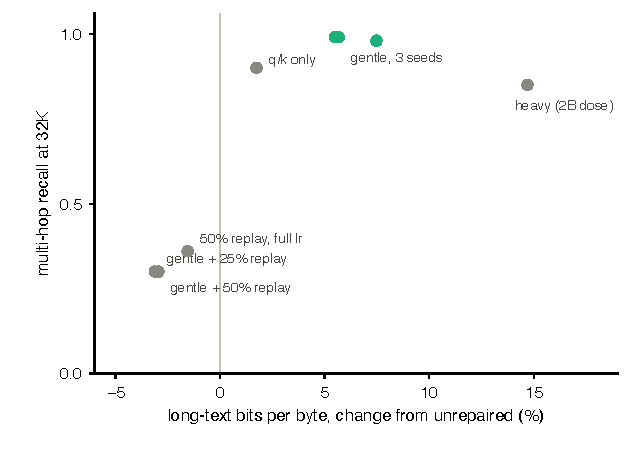
\includegraphics[width=0.62\linewidth]{fig/fig3_tradeoff.pdf}
\caption{8B recipes: the change in long-text bits per byte against two-hop recall at 32K. Each point is one training run; the gentle recipe is shown for three seeds.}
\label{fig:tradeoff}
\end{figure}

\begin{table}[t]
\centering\footnotesize\setlength{\tabcolsep}{4pt}
\caption{8B recipes. Recall at 32K with 100 cases; RULER MK1 with 50; bits per byte on 16K windows of long natural text; HellaSwag accuracy on 500 items (SE 0.022). The unrepaired model: 0.25, 0.09, 0.06, 0.40, 1.008, 0.600.}
\label{tab:recipes}
\begin{tabular}{lcccccc}
\toprule
recipe & 16 random & 16 similar & multi-hop & MK1 & bits/byte & HellaSwag \\
\midrule
heavy: 600 docs, lr $2\times10^{-4}$ & 0.98 & 0.91 & 0.85 & 1.00 & 1.156 & 0.566 \\
gentle: 300 docs, lr $5\times10^{-5}$ (3 seeds) & 1.00 & 0.99 & 0.99 & 0.98 & 1.063--1.083 & 0.584--0.594 \\
gentle + 25\% replay & 1.00 & 0.98 & 0.30 & 0.82 & 0.976 & 0.578 \\
replay 50\%, lr $2\times10^{-4}$ & 0.99 & 0.86 & 0.36 & 0.70 & 0.992 & 0.574 \\
query and key projections only & 1.00 & 0.89 & 0.90 & 0.72 & 1.026 & 0.606 \\
\bottomrule
\end{tabular}
\end{table}

\section{What is known and what is new}
The failure is known. Linear-state models lose multi-key recall at length \citep{zoology2023,based2024,waleffe2024}, RULER detects it \citep{ruler2024}, and an unpaired RULER aggregate for Jet-Nemotron-2B that falls to 46.6 at 32K has been reported \citep{jetlong2026}. A third party has measured Jet-Nemotron-2B at 100\% on single-needle to 256K \citep{attentionamnesia2026}, which agrees with our needle column.

Repair with synthetic retrieval data has precedents. LoLCATs recovered 8K single-needle recall by using passkey data as the conversion data itself \citep{lolcats2024}. Continued training of from-scratch hybrids on recall data improved recall at a few thousand tokens with a small commonsense cost \citep{hybridrecall2025}. Synthetic LoRA data is known to cause forgetting in other settings \citep{syntheticdatahurts2026}.

What we did not find published is the paired measurement of a converted model against the model it came from at 32K with the single-needle versus multi-key split, and a post-hoc adapter that restores multi-key recall at 32K with seed replication, a trained control, transfer to an external benchmark, and the collateral cost measured. The coverage rule, that the repair is bounded by the value types and question types in the data, is shown here from four directions.

Two counter-signals deserve stating. Lizard, a conversion that keeps half its attention layers, reports RULER parity with its teacher to 32K \citep{lizard2025}; the deficit is not universal. And our 8B hybrid keeps half its attention layers yet collapses from 4K, so the number of surviving attention layers does not predict the deficit; what the conversion's training taught them does.

\section{Limits}
Two model families and two scales. One training seed per 8B recipe except the gentle one. UUID values stay unrepaired. The damage checks are ARC-Easy, HellaSwag and bits per byte on one book; a long-context natural task is not included. Qwen2.5-1.5B is Jet-Nemotron's initialisation checkpoint, not a weight-identical base, so part of the 2B gap may predate the attention swap; the 8B pair has the same caveat. The 8B replay runs were on A40 GPUs and the rest on A100s; generation was deterministic within a GPU type and we did not test across types.

\section{Reproducing it}
The harness, the adapter code, the Slurm jobs, every raw completion and the figures are at \url{https://github.com/gottn/recall-guard}. The harness runs against any HuggingFace model in one command and reports a recall curve by length. The repair is \texttt{recall\_guard.cli train}; the evaluation is \texttt{recall\_guard.cli run}. Each table in this paper is rebuilt by one script named in the repository.

\paragraph{Acknowledgements.} Experiments ran on the AAU AI Cloud (CLAAUDIA), Aalborg University. Code, experiment orchestration and drafting were done with Claude (Anthropic) under the author's direction; the author designed the study, reviewed every result and is responsible for the content.

\bibliographystyle{unsrtnat}
\bibliography{refs}
\end{document}
